\documentclass[12pt]{article}
\usepackage[latin1]{inputenc}
\usepackage{amsmath}
\usepackage{amsfonts}
\usepackage{amssymb}
\usepackage{setspace}
\usepackage{enumitem}
\usepackage{verbatim}
\usepackage{amsthm}
\usepackage[table]{xcolor}% http://ctan.org/pkg/xcolor
\usepackage{graphicx}
\usepackage{color}
\usepackage{tabularx}  % for 'tabularx' environment and 'X' column type
\usepackage{algorithm,algorithmic}
\newtheorem{definition}{Definition}
\newtheorem{theorem}{Theorem}
\usepackage{filecontents}
\usepackage{lineno}
\usepackage{authblk}
%\linenumbers
\usepackage[margin=1.in]{geometry}
\usepackage[authoryear]{natbib}
\usepackage[hidelinks]{hyperref}

\title{
Geodetic First Approximation of Size and Timing: \\ User's Guide
}
\author[1]{Brendan Crowell \thanks{crowellb@pnsn.org}}
\author[2]{Ben Baker \thanks{benbaker@isti.com}}
\affil[1]{Pacific Northwest Seismic Network}
\affil[2]{Instrumental Software Technologies, Inc.}
\renewcommand\Authands{ and }
\date{\today}

\begin{document}
\maketitle
\tableofcontents

\clearpage
\section{Introduction}
copy brendan's original manual, note the amazon funding, and add brendan's publications
so people know what to cite  

G-FAST (Geodetic First Approximation of Size and Timing) was developed by Brendan Crowell
as a Python based geodetic earthquake early warning (EEW) module.  Funding from Amazon has
allowed PNSN to developed a compiled-language production variant of G-FAST for integration 
into the USGS's next generation ShakeAlert EEW system.  The software is released under the 
license described in Appendix \ref{s:license}.

Nominally, G-FAST acquires real-time geodetic data and, when triggered by a ShakeAlert
message, activates three geodetic co-seismic inversion suites: a peak ground displacement 
(PGD) inversion, a centroid moment tensor (CMT) inversion, and a CMT driven slip or finite fault
inversion.  The PGD module provides a quick and robust estimate of magnitude.  
The CMT inversion provides a robust estimate of magnitude, depth, and moment tensor
components.  The moment-tensor derived fault planes and depth are then passed onto the
slip inversion which resolves the CMT fault plane ambiguity while providing an 
additional magnitude estimate.  The PGD and slip model are then passed onto the
ShakeAlert decision module as the event unfolds.  

As in the Python implementation, G-FAST still acquires real-time data from the Pacific
Northwest Geodetic Array (PANGA) and, in the EEW context, is triggered on ShakeAlert
messages.  The key differences are now that an Earthworm server is responsible for the
import of PANGA data and the ShakeAlert communication is directly implemented via  
ActiveMQ.  Additionally, G-FAST has been separated into multiple C-libraries to encourage
reuse by groups outside of EEW.  



 

\clearpage
\section{Installation}
This section outlines the GFAST installation procedure.  This consists of two primary steps.
The first step is to install the dependencies.  The second step is to then build GFAST and
link to the dependencies.    

\subsection{Prerequisites}
This section lists the requisite, optional, and workaround libraries for building GFAST.   

\subsubsection{Compilers} 
The following libraries and GFAST can be compiled with a 
C, C++, and Fortran compiler.  It is recommended the compilers have complete 
\href{http://openmp.org/wp/}{OpenMP-4} support for improved code vectorization.  
OpenMP-4 support is realized in GCCv5 and above or Clang 3.9 and above though GFAST has
been successfully built with GCCv4.4.  If using GCCv4 then it is
recommend one set the ``-Wno-unknown-pragmas'' C compiler flag.

\subsubsection{CMake} CMake is used because GFAST is decomposed into many smaller libraries with 
varying dependencies.  This dependency ambiguity is implicitly handled by this automatic 
makefile generator. In addition to generation of makefiles also CMake provides for automatic generation
and execution of unit tests. As with any makefile creation step the correct 
specification of dependencies can be quite painful but, upon successful generation of a
CMakeCache.txt file this activity need not be repeated and subsequent pulls from the git
repository should build without hassle.  CMake is likely available through a package manager
or can be obtained from \url{https://cmake.org/}.  GFAST has been successfully built with
Version 2.6 and above.  

\subsubsection{LAPACK and BLAS} GFAST ultimately aims to solve matrix-vector
equations of the form $\Vert G \textbf{m} = \textbf{d}\Vert_2 $ (LAPACK) or estimate 
data by computing matrix-vector multiplies of the form $\textbf{u} = G \textbf{m}$ (BLAS).  
Moreover, profiling shows that computation of the least-squares problem, particularly in the
finite fault inversion, is the greatest contributor to program execution time.  
Necessarily, one can easily achieve better performance
by using high-performance (commercial) LAPACK and BLAS libraries.  Consequently, it is recommended one
follow the strategy of 
\begin{enumerate}
  \item Check for an existing vendor LAPACK/BLAS implementation.  
  \item If using an Intel processor obtain Intel's Math Kernel Library (MKL) 
        which is freely available at \url{https://software.intel.com/sites/campaigns/nest/}.
        Also, note that MKL contains an implementation of FFTw and may reduce the number of
        dependencies. 
  \item Check a package manager for a pre-built LAPACK and BLAS which are distributed with a
  modified BSD license.
  \item TODO: look for OpenBLAS then, if not found, ATLAS in the CMakeModules if using a 
  package manager's lapacke + blas.      
  \item At last resort obtain and build LAPACK and BLAS from \url{http://www.netlib.org/lapack/}
  which are distributed with a modified BSD license. 
\end{enumerate}

\subsubsection{libGeographic}
This is a library used by GFAST's coordinate tools unit tests.  It may be available through
a package manager or, if need be, obtained from \url{http://geographiclib.sourceforge.net/}.  It is
distributed under the MIT license. 

\subsubsection{iniparser}
This is the utility which parses the GFAST parameter file.  It is available from
\url{https://github.com/ndevilla/iniparser} and is distributed under the MIT license.

\subsubsection{HDF5}
The HDF5 self-describing file format is used for high-performance and portable data archival and
data playback.  HDF5 can be obtained from a package manager or from 
\url{https://www.hdfgroup.org/HDF5/}. 
GFAST appears to work with HDF5 1.18.6.  If static linking to HDF5 then one must additionally 
obtain the zlib compression library.  A zlib implementation is available in Intel's 
Performance Primitives available at \url{https://software.intel.com/sites/campaigns/nest/}.  Zlib
can also be obtained with a package manager or from \url{http://www.zlib.net}.  
Notice that there is no data compression in GFAST disk writes and this step can be avoided by
linking to the shared HDF5 library.  If choosing between IPP and a zlib then note that
IPP improves the performance of ISCL.   Zlib and HDF5 both are distributed with permissive
software licenses.

\subsubsection{libxml2}
The ShakeAlert and QuakeML data products are created with libxml2.  If using GCC then it
is very likely you already have libxml2.  Otherwise, it can be obtained from 
\url{http://xmlsoft.org/}.  libxml2 is distributed under the MIT license. 

\subsubsection{ISCL}
Brendan's initial GFAST implementation was written in Python and made extensive use of 
Numerical Python.  Somewhat fortuitously ISTI had been developing a library targeted 
at expediting the conversion of NumPy laden Python scripts to C via the ISTI Scientific
Computing Library (ISCL).  ISCL is distributed under the Apache-2 license and 
freely available from \url{https://github.com/bakerb845/libiscl}.

\subsubsection{ActiveMQ}
The ShakeAlert earthquake early warning system sends and receives alerts with the ActiveMQ
messaging system.  If one is not using GFAST in earthquake early warning then ActiveMQ
is not necessary.  ActiveMQ additionally depends on libcrypto and libssl.  ActiveMQ is
distributed under the Apache 2 license is available at
\url{http://activemq.apache.org/cms/download.html}. 

\subsubsection{Earthworm}
The real-time GPS data are currently incorporated into GFAST via Earthworm which is
available at \url{http://earthworm.isti.com/trac/earthworm/}.  If not using the real-time
system then Earthworm is not necessary.  Earthworm requires two
additional libraries, RabbitMQ-c and Jansson for import of the GeoJSON which contains the GPS
precise-point-position data.  RabbitMQ-c 
is available at \url{https://github.com/alanxz/rabbitmq-c} and is distributed with an 
MIT license.  Jansson is available at \url{https://github.com/akheron/jansson} and
is distributed with a permissive license. 

\subsubsection{FFTw}
The requirement for this library will be dictated by your linking policy.  If you require 
static linking \emph{and} are not using Intel MKL then to successfully build GFAST you would 
have to obtain FFTw from a package manager or obtain it from \url{http://www.fftw.org/}.
Notice however that no Fourier transforms are computed in GFAST.  Additionally, if static
linking without MKL then FFTw's GPL-2 copyleft will impact GFAST's internal license.
To avoid this complication it is recommended one use MKL or link to the dynamic ISCL library.  

\subsubsection{Cython}
A developmental Python interface is provided through Cython which converts Python to C and is 
available at \url{http://cython.org/} or through a package manager.  This is not required and
at the present time minimally supported.

\subsubsection{cMoPaD}
The moment tensor decompositions are accomplished through a C implementation of 
\href{https://github.com/geophysics/MoPaD}{MoPaD}.  This is distributed with GFAST.  
Because the C implementation is derivative work it must assume MoPaD's original 
LPGL3 license.  This means that one can safely link to the shared MoPaD library without
modifying the GFAST license.  This is reflected in the target link library of the 
src/CMakeLists.txt  file.

\subsection{Building GFAST}

To increase the likelihood that G-FAST can be compiled on multiple platforms (e.g. Linux, 
Windows, OSX) and ease the burden on developers to modify cumbersome makefiles G-FAST 
adopts an automatic makefile generation utility in CMake.  Naively, one can descend 
into G-FAST's src directory and type 
\begin{verbatim}
cmake .
\end{verbatim}  
The CMakeModules will attempt to find the requisite libraries and may be moderately successful
if items are installed in `standard'
locations.  Alternatively, if one would rather specify paths to custom directories
cmake can be used by  
\begin{verbatim}
cmake ./ -DCMAKE_BUILD_TYPE=DEBUG \
      -DCMAKE_INSTALL_PREFIX=./ \
      -DCMAKE_C_FLAGS="-g3 -O2 -fopenmp -Wall -Wno-unknown-pragmas" \
      -DCMAKE_CXX_FLAGS="-g3 -O2" \
      -DAPR_INCLUDE_DIR=path_to_include_apr-1 \
      -DLIBAMQ_INCLUDE_DIR=path_to_include_activemq-cpp-3.8.2 \
      -DLIBAMQ_LIBRARY=path_to_libactivemq-cpp \
      -DLSSL_LIBRARY=path_to_libssl \
      -DLCRYPTO_LIBRARY=path_to_libcrypto \
      -DLAPACKE_INCLUDE_DIR=path_to_lapacke_include \
      -DLAPACKE_LIBRARY=path_to_liblapacke \
      -DLAPACK_LIBRARY=path_to_liblapack \
      -DCBLAS_INCLUDE_DIR=path_to_cblas_include \
      -DCBLAS_LIBRARY=path_to_libcblas \
      -DBLAS_LIBRARY=path_to_libblas \
      -DH5_C_INCLUDE_DIR=path_to_hdf5_include \
      -DH5_LIBRARY=path_to_libhdf5 \
      -DINIPARSER_INCLUDE_DIR=path_to_iniparser_src \
      -DINIPARSER_LIBRARY=path_to_libiniparser \
      -DISCL_INCLUDE_DIR=path_to_iscl_include \
      -DISCL_LIBRARY=path_to_libiscl_static \
      -DGEOLIB_LIBRARY=path_to_libGeographic \
      -DFFTW3_LIBRARY=path_to_libfftw3 \
      -DEW_INCLUDE_DIR=path_to_earthworm_include \
      -DEW_LIBRARY=path_to_earthworm_libew \
      -DLIBXML2_INCLUDE_DIR=path_to_libxml2 \
      -DLIBXML2_LIBRARY=path_to_libxml2
\end{verbatim}
As another example, one can use the MKL and IPP libraries to boost performance 
\begin{verbatim}
cmake ./ -DCMAKE_BUILD_TYPE=DEBUG \
      -DCMAKE_INSTALL_PREFIX=./ \
      -DCMAKE_C_COMPILER=/usr/bin/gcc-5 \
      -DCMAKE_CXX_COMPILER=/usr/bin/c++ \
      -DCMAKE_C_FLAGS="-g3 -O2 -fopenmp -Wall" \
      -DCMAKE_CXX_FLAGS="-g3 -O2" \
      -DAPR_INCLUDE_DIR=path_to_apr \
      -DLIBAMQ_LIBRARY=path_to_libactivemq-cpp \
      -DLSSL_LIBRARY=path_to_libssl \
      -DLCRYPTO_LIBRARY=path_to_libcrypto \
      -DMKL_LIBRARY="mkl;libraries;" \
      -DIPP_LIBRARY="intel;performance;libraries" \
      -DH5_C_INCLUDE_DIR=path_to_hdf5_include \
      -DH5_LIBRARY=path_to_lib_libhdf5 \
      -DINIPARSER_INCLUDE_DIR=path_to_iniparser_src \
      -DINIPARSER_LIBRARY=path_to_libiniparser \
      -DISCL_INCLUDE_DIR=path_to_iscl_include \
      -DISCL_LIBRARY=path_to_libiscl \
      -DGEOLIB_LIBRARY=path_to_libGeographic \
      -DEW_INCLUDE_DIR=path_to_ewinclude \
      -DEW_LIBRARY=path_to_libew \
      -DLIBXML2_INCLUDE_DIR=path_to_libxml2_include \
      -DLIBXML2_LIBRARY=path_to_libxml2
\end{verbatim}

\clearpage
\section{GFAST Library Overview}
This section will outline the GFAST libraries.  Libraries are used extensively 
to emphasize modularity, allow users to customize GFAST to their application 
without incurring the cruft of another GFAST application, and promote a maintainable
software framework whereby software fixes can efficiently propagate to all users.  
The libraries to be introduced are
\begin{itemize}
 \item Subsection \ref{ss:gfastCore}: libgfast\_core for core GFAST modeling and inversion  
 \item add the rest
\end{itemize}

\clearpage
\subsection{GFAST Core Routines}\label{ss:gfastCore}
This section outlines the libgfast\_core utilities which are essential to the expert
earthquake-early warning driver routines.  The six primary utilities are
\begin{itemize}
  \item A properties reader for requisite GFAST modeling parameters.
  \item Waveform processing for computation of peak ground displacement or offsets
  derived from precise-point-position time series data.
  \item PGD inversion of peak ground displacement data computed in the waveform processing.
  \item CMT inversion of offset data computed in the waveform processing.
  \item Finite fault inversion of data computed in the waveform processing.
  \item Coordinate utilities for converting latitude and longitude to and from 
  UTMs\footnote{This directory supersedes the libGeographic ISCL interface as libGeographic 
            has unpredictable behavior when crossing UTM zones that could jeopardize
            program library execution in the Pacific Northwest.}.  
\end{itemize}

\clearpage
\subsection{Data Acquisition}
This section outlines the data acquisition strategy in real-time and playback operations.
To make the real-time acquisition and playback appear integrated to the user a common
HDF5 file format is selected.  For playbacks, a pre-processing program can be used to generate 
a valid input data 
file\footnote{`File' is a generic word in the context of this discussion.  
It is unnecessary and potentially undesirable from a performance standpoint that
the file physically exist in the computer's disk space.  The illusion of keeping 
the file on disk is accomplished by instructing HDF5 to memory map the data 
file during the start-up phase.}
which is queried by a simple API for data in a given a time range.  
Likewise, real-time data is  
written\footnote{The writes can be to memory or disk.}
to an HDF5 file with the same structure as a playback data file and, like in playback mode,
can be queried by the same API as the playback for data in a given time range.

\begin{center}
\begin{figure}
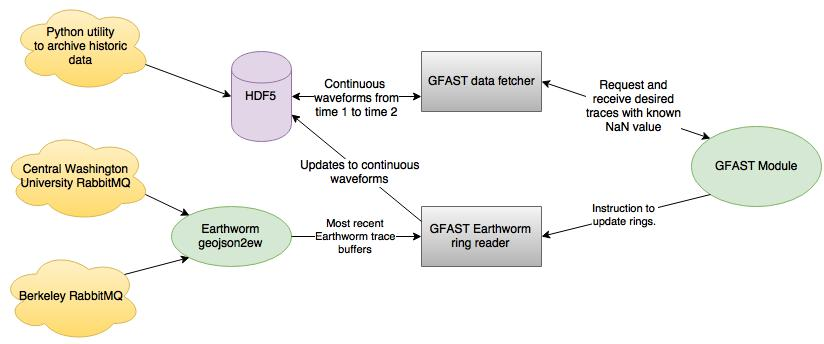
\includegraphics[scale=0.55]{Figs/gfast_dataIO.jpg}
\caption{A depiction of the current data flow.  The goal is to put the data in a common, 
continuous, finite-sized format hereby encapsulated by the HDF5 archive.  
In the context of playbacks the bottom functions are not used.
Hence, it is the same function that queries the HDF5 archive in playback and 
real-time mode and the G-FAST application developer is only exposed to one data 
fetcher API.  The API is very simple in that G-FAST specifies two times, for example 
the event origin time and the current time, and the data is returned with the understanding
some data may be latent or non-existent and have a predetermined value indicating its absence. 
For real-time scenarios the Earthworm acquisition must be configured 
and running prior to launching a G-FAST application.  However, the GPS ring is 
accessed directly by a G-FAST function.  In addition to a playback, a real-time application 
must call the G-FAST ring reader function periodically, say every second, as to refresh the 
HDF5 archive.
}\label{F:gfastDataIO}
\end{figure}
\end{center}

\clearpage
\subsection{XML Output}
This section outlines the three XML data products.  Two XML products, PGD and finite fault, have
defined ShakeAlert schemas.  The third XML product is a QuakeML summary CMT summary for potentially
expediting communication between the tsunami warning centers and NEIC. 

\clearpage
\subsection{HDF5 Output}
This section outlines the HDF5 summary files.  HDF5 is a portable and high performance 
utility which makes it possible to easily archive the results\footnote{Since results are 
encapsulated in data structures the HDF5 files are the data structures after each iteration.}
of GFAST after each iteration thereby providing a snapshot of the GFAST execution and 

\section{Acknowledgements}
This software was developed with funds from the amazon catylyst and government grants a, b, c and d.  

\appendix
\section{License}\label{s:license}
brendan, you have to email the comotion (tech transfer) and see what they want.  
i'm going to guess this software belongs to uw, ideally it is free (as in beer) in
an academic or government setting, uw owns all modifications to the software, the software
is provided as is, and you cannot hold uw liable.  they may settle for a gpl-3 which would 
be a good compromise if the goal is to keep a company from touching it.  this may have
already been decided in the amazon catalyst proposal. 

\end{document}

